% !Mode:: "TeX:DE:UTF-8:Main"
% arara: pdflatex
% arara: pdflatex
% xarara: convert: {density: 160, otheroptions: -dispose previous -delay 10 -loop 0, format: gif}
%magick -density 160 -delay 35 -loop 0 wildwest.pdf wildwest.gif

% slow motion needed!!!!
% https://i.pinimg.com/originals/5a/03/a5/5a03a528bae24b828b93524038952adc.jpg
\documentclass{beamer}

\usepackage{tikzlings,tikzducks,xfp}
\usetikzlibrary{overlay-beamer-styles}
\setbeamertemplate{navigation symbols}{}
\usepackage[T1]{fontenc}

\usepackage{tikzlings}
\usepackage{realhats}
\newcommand\mfactor{0.005}
\begin{document}
\foreach \x in{1,2,...,400}
{
\begin{frame}
\begin{tikzpicture}[remember picture,overlay]
	
% Background image
\node[at=(current page.center)]{%
	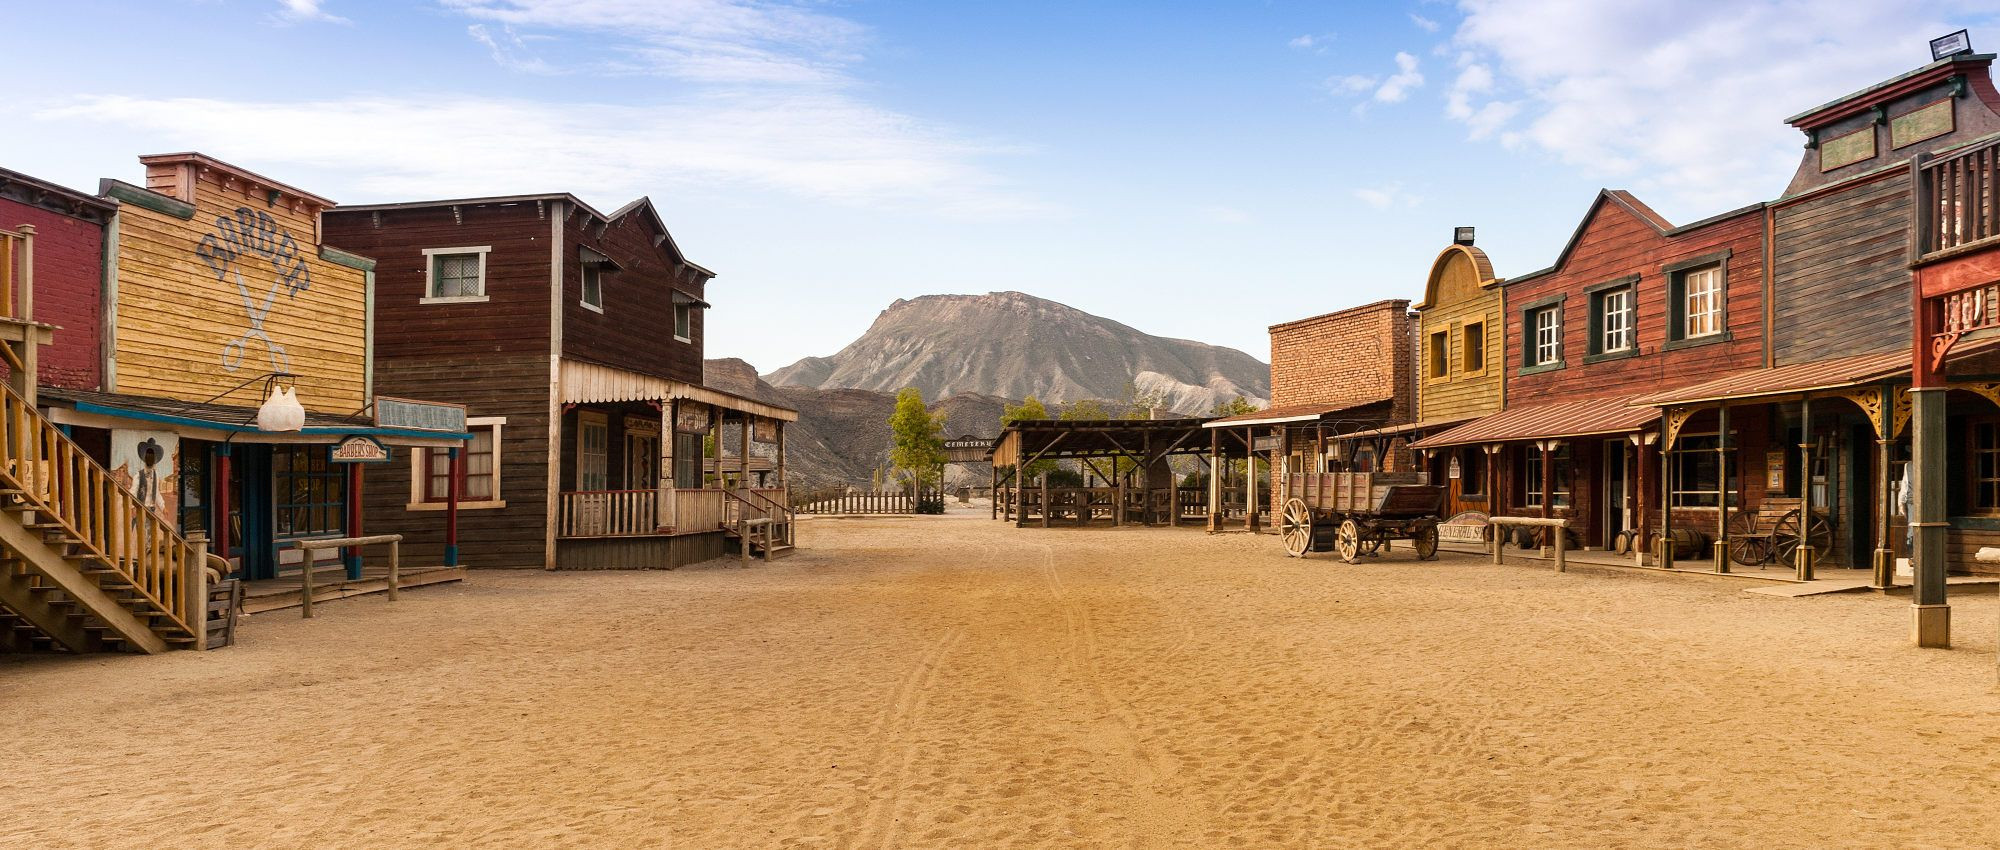
\includegraphics[height=1.05\paperheight]{westerntown}
};	

% Image credit of background
\end{tikzpicture}
\vspace*{\fpeval{4 + \x*\mfactor}cm}

\centering
\scalebox{\fpeval{0.4+\x*\mfactor/10}}{\fontsize{1.7cm}{1.7cm}\selectfont
\stackon[-0.5ex]{\tikz\marmot[body=brown!70!white];}{\hspace{-0.3ex}\includegraphics[width=2ex]{realhats-cowboy}}
\hspace{-2.1cm}\raisebox{-3mm}{
\includegraphics[width=2.5cm,angle=60]{flinte}}}
\end{frame}}


\end{document}